\documentclass{beamer}
\usepackage{beamerthemeshadow}
\usepackage{graphicx}
\usepackage{color}
\usepackage[utf8]{inputenc}
\usepackage{hyperref}
\usepackage[flushleft]{threeparttable}
\usepackage{csquotes}
\usepackage[english,serbian]{babel}
\usetheme{Hannover}
\usecolortheme{wolverine}
\setbeamertemplate{headline}{}


% \definecolor{beamer@green}{rgb}{0.5, 2, 0.5}
% \setbeamercolor{structure}{fg=beamer@green}

\def\dJ{{\fontencoding{T1}\selectfont\dj}}
\def\Dj{{\fontencoding{T1}\selectfont\DJ}}

\begin{document}
\title{Scott Aaronson}
\author[]{Vidak Kozomara, Lazar Perišić, Aleksa Cvetković, \newline \Dj{}or\dJ{}e Milošević}
\institute{Matematički fakultet\\Univerzitet u Beogradu}
\date{
	\footnotesize{Beograd, 2019.}	
}

\begin{frame}
	\thispagestyle{empty}
	\titlepage
\end{frame}

\addtocounter{framenumber}{-1}
%-----------------------------------------------------------------
\begin{frame}[fragile]\frametitle{Skot Aronson}
	\begin{figure}
		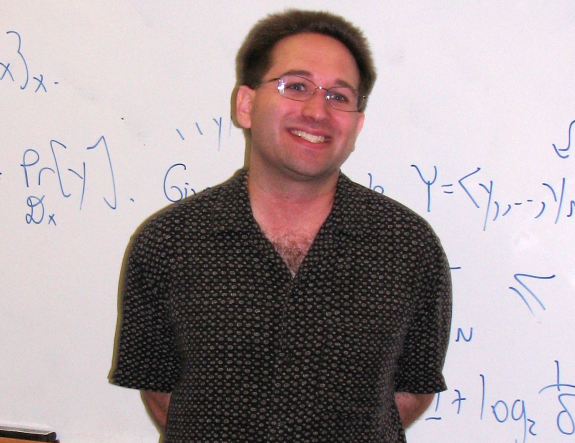
\includegraphics[scale=0.2]{Scott Aaronson.jpg}
		\caption{Skot Aronson}
		\end{figure}
	\begin{displayquote}
		When I was a kid, I wanted to be the founder and ruler of a rationalist space colony, who also wrote video games and invented the first human-level AI and led a children’s liberation movement and discovered the mathematical laws underlying society.
		\footnote{https://blogs.scientificamerican.com/cross-check/scott-aaronson-answers-every-ridiculously-big-question-i-throw-at-him/}
		\end{displayquote}

\end{frame}

\section{Biografija}
\subsection{Kratak uvod}
\begin{frame}[fragile]
    \frametitle{Biografija}
	\begin{itemize}
		\item \textbf{Skot Džoel Aronson} (eng. \textit{Scott Joel Aaronson}) je američki teorijski informatičar i profesor informatike na Univerzitetu u Ostinu, Teksas. Njegove primarne oblasti istraživanja su mogućnosti i limiti kvantnih računara kao i računarska teorija složenosti.
	\end{itemize}
\end{frame}
%------------------------------------------------------------------------
\subsection{Mladost i obrazovanje}
\begin{frame}
	\frametitle{Mladost i obrazovanje} 
%	\tableofcontents[hidesubsections]
	\begin{itemize}
	    \item Ro\dJ{}en u Filadelfiji, SAD
	    \item Boravak u Aziji
	    \item Dana Moškovic
	    \item Kornel Univerzitet
	    \item Berkli Univerzitet
	    
	\end{itemize}
\end{frame}
%-----------------------------------------------------------------------

\subsection{Karijera}
\begin{frame}[fragile]\frametitle{Karijera}
	\begin{itemize}	
		\item Njegova primarna oblast je kvantno programiranje i računarska teorija složenosti.
		\item Pored karijere u obrazovanju, Skot Aronson je radio i za neke kompanije poput: VMware, Pivotal Software Inc, Greylock Partners, Cloudera Inc, Medallia Inc
	\end{itemize}
\end{frame}

\subsection{Nagrade}
\begin{frame}[fragile]\frametitle{Nagrade}
	\begin{itemize}	
		\item Jedan od dva dobitnika nagrade Alan T. Vaterman za 2012. godinu
		\item Nagrada za najbolji rad u računarstvu u Rusiji 2011. godine za rad "Ekvivalentnost uzrokovanja i pretraživanja"
		\item 2017. Simons istražitelj
	\end{itemize}
\end{frame}


\section{Zanimljivosti}
\subsection{Marketinški plagijat}
\begin{frame}[fragile]\frametitle{Marketinški plagijat}
	\begin{itemize}
		\item<2-> U oktobru 2007. godine optužio marketinšku agenciju Lav Komunikejšns (eng. \textit{Love Communications})
		\item<2-> Prisvojili deo njegovog predavanja u jednoj marketinškoj kampanji za Riko (eng. \textit{Ricoh})
		\item<3-> Predlaže nagodbu
		\item<4-> Prihvataju nagodbu ali sa mnogo manjom odštetom
	\end{itemize}
\end{frame}

\begin{frame}[fragile]\frametitle{Marketinški plagijat}
	\begin{itemize}
		\item<1-> Prihvata nagodbu od 5000 dolara
		\item<2-> Doniran novac organizacijama koje popularizuju nauku u Australiji
		\item<3-> Generalni direktor Lav Komunikejšnsa je izjavio da su verovatno trebali da ga pitaju 
		pre nego što su iskoristili njegove reči ali da ne misle da su prekršili autorska prava
		
	\end{itemize}
\end{frame}

\section{Literatura}
\begin{frame}[fragile]\frametitle{Literatura}
	\begin{itemize}
	\item \begin{verbatim} https://sr.wikipedia.org/wiki/Skot_Aronson \end{verbatim}
	\end{itemize}
\end{frame}

\begin{frame}[fragile]\frametitle{Zahvalnica}
	\thispagestyle{empty}
	\begin{center}
		{\Huge Hvala na paznji}
	\end{center}	
\end{frame}
%-----------------------------------------------------------------------

% \begin{frame}[fragile]\frametitle{Kako ljudi uče?}
% 	\begin{itemize}	
		
% 	\end{itemize}
% \end{frame}


% \begin{frame}[fragile]\frametitle{Opšte preporuke za dobru usmenu prezentaciju}
% 	\begin{itemize}	
			
% 	\end{itemize}
% \end{frame}

% \begin{frame}[fragile]\frametitle{Opšte preporuke za dobru usmenu prezentaciju}
% 	\begin{itemize}	
		
% 	\end{itemize}
% \end{frame}

% \begin{frame}[fragile]\frametitle{Opšte preporuke za dobru usmenu prezentaciju}
% 	\begin{itemize}		
% 		\item Nikada nemojte čitati ceo tekst sa papira ili sa ekrana
% 		\item Trudite se da nemate konfuzne izjave. Izbegavajte suprotnosti
% 				\item Podaci u prezentaciji moraju teći logičkim sledom
% 		-- na slajdove pišite samo nužne informacije, ostalo dodajte usmenim izlaganjem
%      	\item Neka prelazi iz jedne na drugu temu budu ,,glatki``		
% 		\item Obratite pažnju na vremensko trajanje prezentacije; ako prezentacija traje predugo, i vi i publika gubite koncentraciju
% 		\item Budite spremni da podelite sa publikom ono što znate ali
% 		i da čujete ono što ne znate
% 		\item Pažljivo saslušajte komentare publike. Pokušajte
% 		da objasnite publici ono što ste želeli da kažete		
% 	\end{itemize}
% \end{frame}

% \begin{frame}[fragile]\frametitle{Struktura prezentacije}
% 	\begin{itemize}	
% 		\item  Uvod
% 		\begin{itemize}
% 			\item Pozdravite publiku
% 			\item Pohvalite organizaciju doga\d{}aja
% 			\item Pokažite dobre manire
% 		\end{itemize}
% 		\item Početak
% 		\begin{itemize}
% 			\item Ako je moguće, pokušajte da se povežete sa prethodnim govornikom
% 			\item Postavite ,,okvir`` prezentacije
% 			\item Privucite pažnju nekom ubedljivom pričom ili
% 			anegdotom
% 			\item Definišite glavne teme, ne više od tri
% 		\end{itemize}		
% 	\end{itemize}
% \end{frame}

% \begin{frame}[fragile]\frametitle{Struktura prezentacije}
% 	\begin{itemize}			
% 		\item Središnji deo
% 		\begin{itemize}
% 			\item Prikažite kratko šta su drugi uradili na temu koju
% 			prezentujete
% 			\item Prikažite svoje rezultate i doprinose
% 			\item Nemojte samo prikazivati sirove formule. Pokušajte da ih nekako
% 			obrazložite
% 		\end{itemize}
% 		\item Kraj
% 		\begin{itemize}
% 			\item Rekapitulacija. Ponovite glavne teme
% 			\item Ponovite ključne rezultate
% 			\item Navedite literaturu koju ste koristili u istraživanju
% 			\item Poslednjim slajdom zahvalite publici na pažnji		
% 		\end{itemize}		
% 	\end{itemize}
% \end{frame}



% \begin{frame}[fragile]\frametitle{Kreiranje slajdova i prezentacija}
% 	\begin{itemize}	
% 		\item \LaTeX{} se može koristiti za kreiranje atraktivnih slajdova i prezentacija	
% 		\item Osnovna podrška za kreiranje slajdova u \LaTeX{}-u postoji u vidu klase \verb"slides"		
% 		\item Ova klasa podrazumeva korišćenje velikih, bez-serifnih slova čime se dobija dokument koji je pogodan za prikazivanje na projektoru		
% 		\item Pored ovoga, klasa \verb"slides" ne pruža nikakvu dodatnu podršku za kreiranje prezentacija		
% 		\item \textcolor{beamer@darkred}{Primer 13}
% 	\end{itemize}
% \end{frame}

% \begin{frame}[fragile]\frametitle{Napredna sredstva za kreiranje prezentacija}
% 	\begin{itemize}	
% 		\item Namenske komande koje olakšavaju rad sa slajdovima mogu se naći u dodatnim \LaTeX{} paketima		
% 		\item Postoji veći broj takvih paketa sa sličnim mogućnostima		
% 		\item Ovde će biti predstavljen paket \verb"beamer" koji ima odličnu podršku za kreiranje
% 		dinamičkih prezentacija \footnotesize (\url{http://tug.ctan.org/macros/latex/contrib/beamer/doc/beameruserguide.pdf}) \normalsize		
% 		\item Predvi\d{}eno je da se dokumenti kreirani uz pomoć ovog paketa prevode u pdf
% 		format radi prikazivanja prezentacije na ekranu, pri čemu
% 		\verb"beamer" nudi čitav niz efekata za postupni prikaz sadržaja, kao i za prelaz izme\d{}u dva slajda		
% 		\item Paket omogućava i generisanje slajdova za prikaz na
% 		projektoru, ili generisanje štampane verzije prezentacije
% 	\end{itemize}
% \end{frame}

% \begin{frame}[fragile]\frametitle{Napredna sredstva za kreiranje prezentacija}
% 	\begin{itemize}	
% 		\item Paket \verb"beamer" sadrži definiciju istoimene klase dokumenata		
% 		\item \LaTeX{} dokumenti koji predstavljaju prezentacije kreirane korišćenjem ovog paketa treba da
% 		počnu sa:
		
% 		\verb"\documentclass[opcije]{beamer}"
		
% 		\item Stil prezentacije je odre\d{}en tzv. temom, koja se u preambuli dokumenta
% 		zadaje komandom: \verb"\usetheme{tema}"		
% 		\item Tema odre\d{}uje boju pozadine i teksta, fontove kojima će biti
% 		ispisani naslovi ili običan tekst, grafiku koja će biti prikazana na svakom slajdu
% 		i tako dalje		
% 		\item Na raspolaganju je veliki broj podrazumevanih tema, koje su nazvane po gradovima,
% 		na primer \verb"Antibes", \verb"Berlin", \verb"Copenhagen", \verb"Frankfurt", \verb"Madrid", \verb"Szeged" i \verb"Warsaw"
% 	\end{itemize}
% \end{frame}

% \begin{frame}[fragile]\frametitle{Napredna sredstva za kreiranje prezentacija}
% 	\begin{itemize}	
% 		\item	Navedene teme u potpunosti odre\d{}uju stil prezentacije, a 
% 		pojedinačni aspekti prezentacije se mogu kontrolisati tzv. podtemama, 
% 		koje se mogu svrstati u četiri kategorije navedene u tabeli: 		
% 		\begin{tabular}{|l|l|}
% 			\hline	
% 			\footnotesize	komanda & \footnotesize značenje\\
% 			\hline
% 			\hline \footnotesize
% 			\footnotesize   \verb"\useoutertheme{podtema}" &\footnotesize kontroliše dekoracije na slajdovima \\
% 			\footnotesize	\verb"\useinnertheme{podtema}" &\footnotesize kontroliše izgled glavnog dela na slajdovima \\
% 			\footnotesize	\verb"\usefonttheme{podtema}" &\footnotesize kontroliše fontove na slajdovima \\
% 			\footnotesize	\verb"\usecolortheme{podtema}" &\footnotesize kontroliše boje na slajdovima\\
% 			\hline
% 		\end{tabular}
% 	\end{itemize}
% \end{frame}

% \begin{frame}[fragile]\frametitle{Napredna sredstva za kreiranje prezentacija}
% 	\begin{itemize}	
% 		\item Još finija kontrola nad pojedinim aspektima prezentacije ostvaruje se komandama
% 		\verb"\setbeamertemplate", \verb"\setbeamerfont" i \verb"\setbeamercolor"		
% 		\item	Tako se na primer ikonice za navigaciju kroz prezentaciju, koje bivaju automatski generisane u svakoj
% 		\verb"beamer" prezentaciji, eliminišu komandom: \verb"\setbeamertemplate{navigation symbols}{}"		
% 		\item	Klasa \verb"beamer" redefiniše neke standardne \LaTeX{} komande  		
% 	\end{itemize}
% \end{frame}

% \begin{frame}[fragile]\frametitle{Napredna sredstva za kreiranje prezentacija}
% 	\begin{itemize}	
% 			\item	Komande koje se mogu navesti u preambuli dokumenta date su u tabeli:			
% 			\begin{tabular}{|l|l|}
% 				\hline	
% 				\footnotesize	komanda & \footnotesize značenje\\
% 				\hline
% 				\hline \footnotesize
% 				\footnotesize \verb"title" &\footnotesize naslov prezentacije \\
% 				\footnotesize \verb"subtitle" &\footnotesize podnaslov prezentacije \\
% 				\footnotesize \verb"author" &\footnotesize autor (odnosno autori) prezentacije \\
% 				\footnotesize \verb"institute" &\footnotesize ime institucije sa koje dolazi autor\\
% 				\footnotesize \verb"date"&\footnotesize datum\\
% 				\hline
% 			\end{tabular}
% 			\item Komanda \verb"\titlepage" na osnovu vrednosti zadatih u preambuli dokumenta kreira 
% 			naslov prezentacije unutar datog slajda
% 	\end{itemize}
% \end{frame}

% \begin{frame}[fragile]\frametitle{Napredna sredstva za kreiranje prezentacija}
% 	\begin{itemize}	
% 		\item Pojedinačni slajdovi u dokumentu se navode unutar okruženja \verb"frame"		
% 			\item Ovo okruženje počinje komandom:		
% 		\verb"\begin{frame}{naslov}"
			
% 			a završava se komandom:
			
% 			\verb"\end{frame}"		
% 		\item	Argument \verb"naslov" u komandi kojom počinje okruženje predstavlja nisku koja će
% 		biti ispisana kao naslov slajda
% 	\end{itemize}
% \end{frame}

% \begin{frame}[fragile]\frametitle{Napredna sredstva za kreiranje prezentacija}
% 	\begin{itemize}	
% 		\item Različiti efekti prelaza sa jednog slajda na drugi mogu se postići stavljanjem odgovarajućih komandi unutar
% 		\verb"frame" okruženja 		
% 		\item	Neke od tih komandi su:
% 		\begin{itemize}
% 			\item  \verb"\transdissolve" --- tekući slajd se preliva u naredni slajd
% 			\item \verb"\transwipe" --- linija ,,briše`` ekran otkrivajući naredni slajd ili
% 			\item \verb"\transboxout" --- naredni slajd se pomalja preko tekućeg počev od centralnog dela slajda prema
% 			ivicama
% 		\end{itemize}		
% 		\item	Podrazumevani efekat je da naredni slajd neposredno zamenjuje tekući slajd 		
% 		\item	Trajanje efekta se može precizirati \verb"\transduration" komandom unutar \verb"frame" okruženja
% 	\end{itemize}
% \end{frame}

% \begin{frame}[fragile]\frametitle{Napredna sredstva za kreiranje prezentacija}
% 	\begin{itemize}	
% 		\item Unutar okruženja
% 		\verb"frame"
% 		mogu se koristiti sve \LaTeX{} komande za rad sa
% 		tekstom		
% 		\item	Na slajdovima se često koristi okruženje \verb"itemize"		
% 		\item	Izgled takozvanih \verb"bullet"-a, koji označavaju stavke liste na različitim nivoima
% 		hijerarhije, može se podešavati pomenutim komandama \verb"\setbeamertemplate", \verb"\setbeamerfont" i \verb"\setbeamercolor"
% 		\item \textcolor{beamer@darkred}{Primer 14}
% 	\end{itemize}
% \end{frame}

% \begin{frame}[fragile]\frametitle{Napredna sredstva za kreiranje prezentacija}
% 	\begin{itemize}	
% 		\item  Moguće je koristiti i animirane efekte za postupni prikaz sadržaja slajda		
% 		\item Ovakav efekat je najjednostavnije postići umetanjem komande \verb"\pause"
% 		na jednom ili više mesta unutar \verb"frame" okruženja		
% 		\item	Sadržaj slajda tada tokom prezentacije biva prikazan inkrementalno, i to prvo samo deo slajda do mesta gde je
% 		umetnuta prva komanda \verb"\pause", zatim se komandom za prelazak na naredni
% 		slajd u prezentaciji prikazuje i deo slajda do mesta gde je umetnuta naredna komanda
% 		\verb"\pause", i tako dalje.		
% 	\end{itemize}
% \end{frame}

% \begin{frame}[fragile]\frametitle{Napredna sredstva za kreiranje prezentacija}
% 	\begin{itemize}	
% 		\item Preciznija kontrola nad ovim efektom se može postići \verb"\onslide<lista>" komandom		
% 		\item Slajd se i u ovom slučaju prikazuje inkrementalno, te komanda za
% 		prelazak na naredni slajd u prezentaciji ovde aktivira deo po deo slajda		
% 		\item	Brojevi u listi koja se zadaje u \verb"\onslide" komandi označavaju u kom segmentu
% 		prikaza slajda će tekst koji sledi komandu biti vidljiv. 		
% 		\item	Brojevi u listi se razdvajaju zarezima, a niz brojeva je moguće kraće zapisati u obliku
% 		\verb"m-n", gde je \verb"m" prvi broj u nizu, a \verb"n" poslednji		
% 		\item	Ako se u \verb"\onslide" komandi lista izostavi, onda će tekst koji sledi biti vidljiv u svakom segmentu prikaza 
% 		datog slajda
% 	\end{itemize}
% \end{frame}

% \begin{frame}[fragile]\frametitle{Napredna sredstva za kreiranje prezentacija}
% 	\begin{itemize}	
% 		\item Ukoliko je na primer sadržaj slajda definisan na sledeći način:		
% 		\footnotesize
% 		\begin{verbatim}
% 			\onslide
% 			Suglasnici su: \\
% 			\onslide<1,2,3>b \\
% 			\onslide<2,3>c \\
% 			\onslide<3>d\\
% 			\onslide
% 			Samoglasnici su: \\
% 			\onslide<1-3>a \\
% 			\onslide<2-3>e \\
% 			\onslide<3>i
% 		\end{verbatim} \normalsize		
% 		tada će u prvom koraku prikaza slajda biti vidljiva slova \verb"b" i \verb"a", u drugom koraku
% 		će biti dodata slova \verb"c" i \verb"e", a u trećem koraku i slova \verb"d" i
% 		\verb"i", dok će tekst ,,Suglasnici/samoglasnici su:`` biti vidljiv sve vreme prikaza slajda
% 		\item \textcolor{beamer@darkred}{Primer 15}
% 	\end{itemize}
% \end{frame}
\end{document}
